\documentclass[a4paper]{article}
\usepackage[utf8x]{inputenc}
\usepackage[T1,T2A]{fontenc}
\usepackage[russian]{babel}
\usepackage{hyperref}
\usepackage{indentfirst}
\usepackage{listings}
\usepackage{color}
\usepackage{here}
\usepackage{array}
\usepackage{multirow}
\usepackage{graphicx}

\usepackage{caption}
\renewcommand{\lstlistingname}{Программа} % заголовок листингов кода

\usepackage{listings}
\lstset{ %
extendedchars=\true,
keepspaces=true,
language=bash,					% choose the language of the code
basicstyle=\footnotesize,		% the size of the fonts that are used for the code
numbers=left,					% where to put the line-numbers
numberstyle=\footnotesize,		% the size of the fonts that are used for the line-numbers
stepnumber=1,					% the step between two line-numbers. If it is 1 each line will be numbered
numbersep=5pt,					% how far the line-numbers are from the code
backgroundcolor=\color{white},	% choose the background color. You must add \usepackage{color}
showspaces=false				% show spaces adding particular underscores
showstringspaces=false,			% underline spaces within strings
showtabs=false,					% show tabs within strings adding particular underscores
frame=single,           		% adds a frame around the code
tabsize=2,						% sets default tabsize to 2 spaces
captionpos=b,					% sets the caption-position to bottom
breaklines=true,				% sets automatic line breaking
breakatwhitespace=false,		% sets if automatic breaks should only happen at whitespace
escapeinside={\%*}{*)},			% if you want to add a comment within your code
postbreak=\raisebox{0ex}[0ex][0ex]{\ensuremath{\color{red}\hookrightarrow\space}}
}

\usepackage[left=2cm,right=2cm,
top=2cm,bottom=2cm,bindingoffset=0cm]{geometry}

\begin{document}	% начало документа

\begin{titlepage}	% начало титульной страницы

	\begin{center}		% выравнивание по центру

		\large Санкт-Петербургский Политехнический Университет Петра Великого\\
		\large Институт компьютерных наук и технологий \\
		\large Кафедра компьютерных систем и программных технологий\\[6cm]
		% название института, затем отступ 6см
		
		\huge Программирование\\[0.5cm] % название работы, затем отступ 0,5см
		\large Отчет по лабораторной работе \\[0.1cm]
		\large Игра "Морской бой"\\[5cm]

	\end{center}


	\begin{flushright} % выравнивание по правому краю
		\begin{minipage}{0.25\textwidth} % врезка в половину ширины текста
			\begin{flushleft} % выровнять её содержимое по левому краю

				\large\textbf{Работу выполнила:}\\
				\large Власова А.В.\\
				\large {Группа:} 13501/4\\
				
				\large \textbf{Преподаватель:}\\
				\large Вылегжанина К.Д.

			\end{flushleft}
		\end{minipage}
	\end{flushright}
	
	\vfill % заполнить всё доступное ниже пространство

	\begin{center}
	\large Санкт-Петербург\\
	\large \the\year % вывести дату
	\end{center} % закончить выравнивание по центру

\thispagestyle{empty} % не нумеровать страницу
\end{titlepage} % конец титульной страницы

\vfill % заполнить всё доступное ниже пространство








% Содержание
\tableofcontents
\newpage



\section{Игра Морской бой}

Морской бой - это традиционная настольная игра, известная каждому человеку с детства. Несмотря на то, что Морской бой существует уже больше 80 лет, эта игра остаеся популярной в наши дни.

\subsection{Задание}

Реализовать проект Морской бой, позволяющий вести игру между человеком и компьютером по базовым правилам.

\subsection{Концепция}

Готовое приложение дает возможность пользователю играть в Морской бой с компьютером в соответствии со стандартными правилами. Программа обладает графическим интерфейсом.

\subsection{Правила игры}

Поле каждого игрока представляет собой квадрат 10х10, на котором размещаются корабли. Поле содержит числовые и буквенные координаты (по вертикали числа от 1 до 10,а по горизонтали буквы от A до J). Для классической игры используются 4 однопалубных корабля, 3 двупалубных, 2 трехпалубных и 1 четырехпалубный корабль. Их размещают внутри игрового поля. По правилам, корабли не должны соприкасаться. Размещать корабли можно как горизонтально, так и вертикально.

Рядом со своим полем игрок видит поле противника, где крестиком отмечает попадания по чужим кораблям. Попавший игрок делает ещё один ход.

\subsubsection{Игровой процесс}

\begin{itemize}

\item Игрок, выполняющий ход, называет координату, на которой, по его мнению, располагается корабль соперника. Например, А3.
\item При промахе игрок получает от противника сообщение «Мимо!», при попадании «Ранил» или «Убил».
\item Игра продолжается до потопления всех кораблей одного из игроков.

\end{itemize}

\subsubsection{Нарушения}

\begin{itemize}

\item Количество кораблей не соответствует правилам
\item Корабли расположены вплотную друг к другу
\item Изменен размер поля
\item Указаны неправильные координаты

\end{itemize}

\subsection{Минимально работоспособный продукт}

Минимальным работоспособным продуктом является консольное приложение, позволяющее вести игру между человеком и компьютером по базовым правилам.

\subsection{Диаграмма прецедентов использования}

\begin{figure}[H]
	\begin{center}
		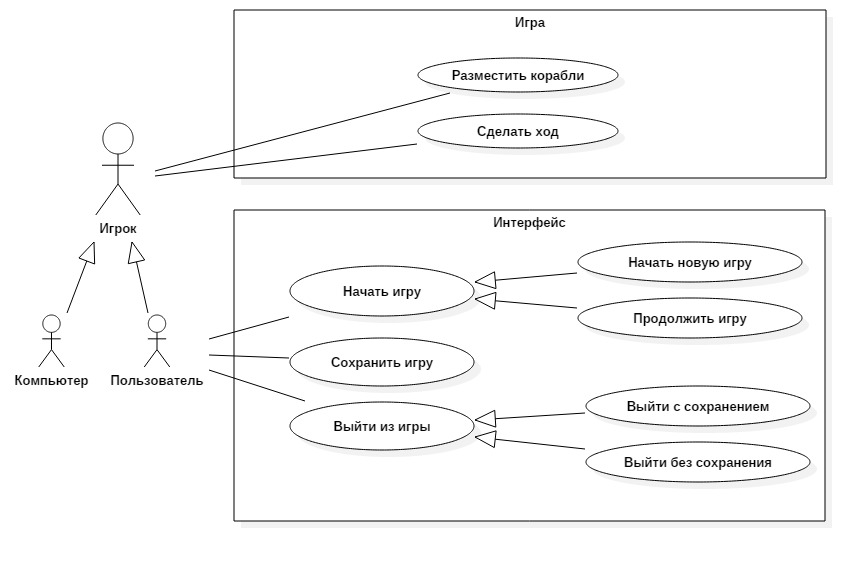
\includegraphics[scale=0.7]{Diagrams/UseCaseDiagram.png}
		\caption{Диаграмма прецедентов} 
		\label{pic:pic_name} % название для ссылок внутри кода
	\end{center}
\end{figure}

На рис.1 изображена диаграмма прецедентов использования. Пользователю дается возможность начинала новой игры, сохранения текущего состояния партии и продолжения сохраненных партий. Во время игрового процесса игроки могут расставлять свои корабли и делать ходы.

\subsection{Выводы}

В данном разделе определены концепция готового приложения и минимальный работоспособный продукт. Также приведены стандартные правила игры в Морской бой, рассмотрен игоровой процесс и основные нарушения. Кроме того, в разделе представлена диаграмма прецедентов использования. 


\section{Проектирование приложения, реализующего игру Морской бой}

\subsection{Выделенные подпроекты}

В процессе проектирования приложения было выделено четыре подпроекта.

\begin{itemize}

\item \textbf{Core}

Библиотека приложения, представляющая игровую модель.

\item \textbf{Console}

Консольное приложение, обеспечивающее взаимодействие пользователя с ядром через консоль.

\item \textbf{GUI}

Графическое приложение, предоставляющее пользователю графический интерфейс для взаимодействия с ядром приложения.

\item \textbf{Test}

Автоматические тесты, созданные для тестирования основной функциональности ядра.

\end{itemize}

\subsection{Описание интерфейса библиотеки}

Интерфейс библиотеки выделен в отдельный класс \textbf{GameAPI}, содержащий в себе следующие методы:

\begin{itemize}

\item Метод, позволяющий совершить ход компьютера

\textbf{bool makeComputerMove() noexcept;}

\item Метод, позволяющий совершить ход пользователя

\textbf{bool makeUserMove(int x, int y) noexcept;}

\item Метод, возвращающий указатель на поле игрока

\textbf{Field* getUserField() const noexcept;}

\item Метод, возвращающий указатель на поле компьютера

\textbf{Field* getComputerField() const noexcept;}

\item Метод, позволяющий разместить корабли пользователя

\textbf{void placeUserShip(int x, int y, int lenght, shipLocation location) noexcept;}

\item Метод, позволяющий разместить корабли автоматически

\textbf{void placeShipsAutomatically(Field* field) noexcept;}

\item Метод, позволяющий узнать, все ли корабли одного поля разрушены

\textbf{bool allShipsDestroyed(Field* field) noexcept;}

\end{itemize}

\subsection{Диаграмма компонентов}

\begin{figure}[H]
	\begin{center}
		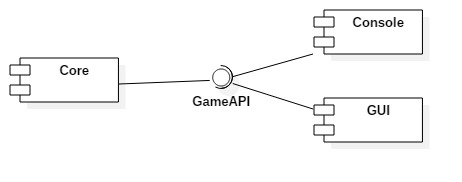
\includegraphics[scale=0.7]{Diagrams/ComponentDiagram.jpg}
		\caption{Диаграмма компонентов} 
		\label{pic:pic_name} % название для ссылок внутри кода
	\end{center}
\end{figure}

На рис.2 представлена диаграма компонентов, отображающая зависимости между основными компонентами приложения.

\subsection{Выводы}

В данном разделе рассмотрен процесс проектирования приложения. Описаны выделенные подпроекты, а также методы класса textbf{GameAPI}, содержащего интерфейс ядра. Помимо этого, в разделе представлена диаграмма компонентов приложения. 

\section{Реализация игры Морской бой}

\subsection{Среда разработки}

Операционная система: Windows 8

Среда разработки: Qt Creator 3.5.1

Компилятор: MinGW 4.9.2

\subsection{Выделенные классы}

В библиотеке были выделены следующие классы:
\begin{itemize}

\item \textbf{Cell}  - содержит основную информацию об одной клетке игрового поля. Позволяет определить координаты клетки и ее статус.

\item \textbf{Ship} - содержит основную информацию о корабле. Позволяет определить его расположение на игровом поле, статус и количество палуб.

\item \textbf{Field} - обеспечивает взаимодействие с игровым полем одного из игроков. Содержит информацию обо всех кораблях поля, о количестве разрушенных кораблей, обеспечивает возможность автоматического и ручного размещения кораблей.

\item \textbf{GameAPI} - интерфейс ядра. Описан в разделе 2.1 

\end{itemize}

В подпроекте \textbf{Console} выделен единственный класс \textbf{Application}, обеспечивающий взаимодействие пользователя с ядром через консоль. Содержит в себе методы, позволяющие выводить поля пользователя и компьютера в консоль, размещать корабли и вести игровой процесс.\\


Проект \textbf{GUI} содержит в себе три класса:

\begin{itemize}

\item \textbf{MainWindow} - главное окно графического приложения, отображающее игровое меню.

\item \textbf{GameWindow} - окно, в котором происходит игровой процесс.

\item \textbf{ResultWindow} - окно, отображащее победителя игры. 

\end{itemize}

\subsection{Примеры работы консольного приложения}

Для демонстрации работы консольного приложения ниже представлены снимки экрана работающего приложения.

\begin{figure}[H]
	\begin{center}
		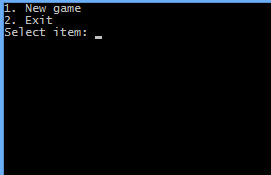
\includegraphics[scale=0.7]{screen/console_menu.png}
		\caption{Главное меню} 
		\label{pic: console main menu} % название для ссылок внутри кода
	\end{center}
\end{figure}

На рис.3 представлено главное меню консольного приложения. 

\begin{figure}[H]
	\begin{center}
		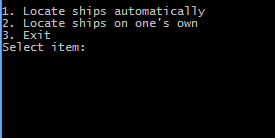
\includegraphics[scale=0.7]{screen/console_locate_ships_menu.png}
		\caption{Меню выбора способа расстановки кораблей} 
		\label{pic:pic_name} % название для ссылок внутри кода
	\end{center}
\end{figure}

На рис.4 показано меню, позволяющее пользователю выбрать способ расстановки своих кораблей: автоматический или ручной.

\begin{figure}[H]
	\begin{center}
		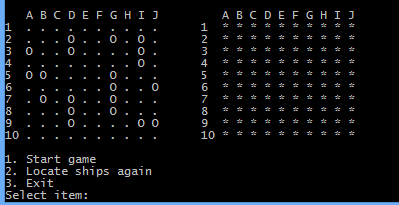
\includegraphics[scale=0.6]{screen/console_start_game.png}
		\caption{Начало игры} 
		\label{pic:pic_name} % название для ссылок внутри кода
	\end{center}
\end{figure}

На рис.5 изображены поля с автоматически расставленными кораблями. После размещения кораблей пользователю предлагается начать игру или расставить корабли заново.

\begin{figure}[H]
	\begin{center}
		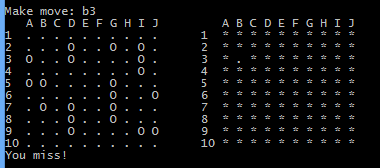
\includegraphics[scale=0.6]{screen/console_user_move.png}
		\caption{Ход пользователя} 
		\label{pic:pic_name} % название для ссылок внутри кода
	\end{center}
\end{figure}

На рис.6 показан пример хода пользователя. 

\begin{figure}[H]
	\begin{center}
		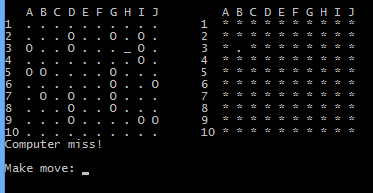
\includegraphics[scale=0.6]{screen/console_computer_move.png}
		\caption{Ход компьютера} 
		\label{pic:pic_name} % название для ссылок внутри кода
	\end{center}
\end{figure}

На рис.7 показан пример рандомного хода компьютера.

\begin{figure}[H]
	\begin{center}
		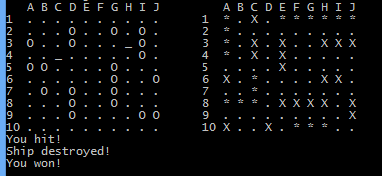
\includegraphics[scale=0.6]{screen/console_winner.png}
		\caption{Вывод победителя} 
		\label{pic:pic_name} % название для ссылок внутри кода
	\end{center}
\end{figure}

Когда все корабли одного из игроков разрушены, выводится победитель игры. Пример вывода победителя представлен на рис.8.

\newpage

\subsection{Пример работы графического приложения}

Ниже приведены снимки экрана для демонстрации работы графического приложения.

\begin{figure}[H]
	\begin{center}
		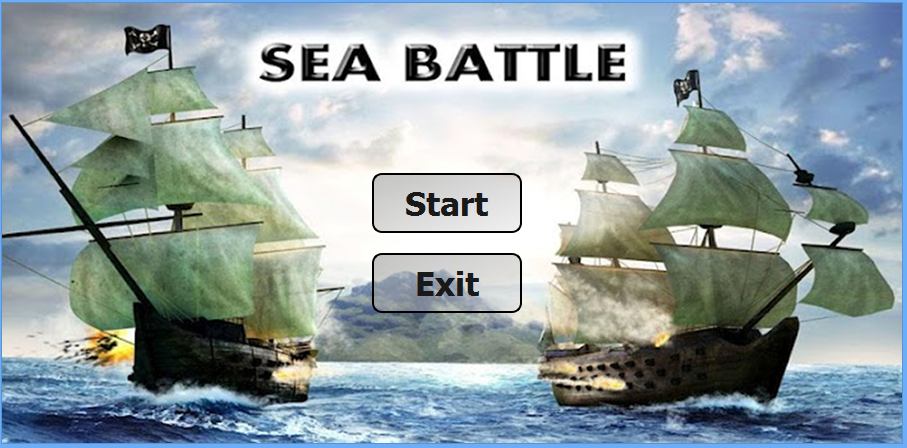
\includegraphics[scale=0.5]{screen/GUI_menu.png}
		\caption{Главное меню} 
		\label{pic:pic_name} % название для ссылок внутри кода
	\end{center}
\end{figure}

На рис.9 отображено главное меню графического приложения.

\begin{figure}[H]
	\begin{center}
		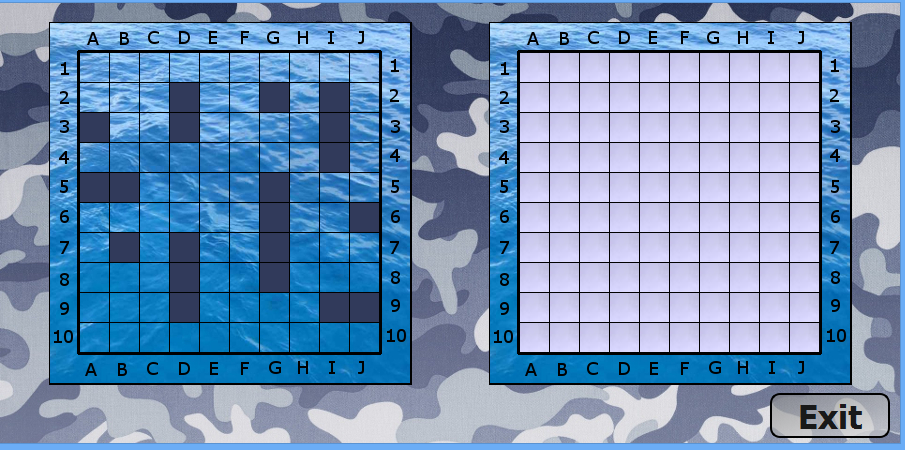
\includegraphics[scale=0.5]{screen/GUI_start.png}
		\caption{Начало игры} 
		\label{pic:pic_name} % название для ссылок внутри кода
	\end{center}
\end{figure}

На рис.10 показано, как выглядят игровые поля в начале игры.

\begin{figure}[H]
	\begin{center}
		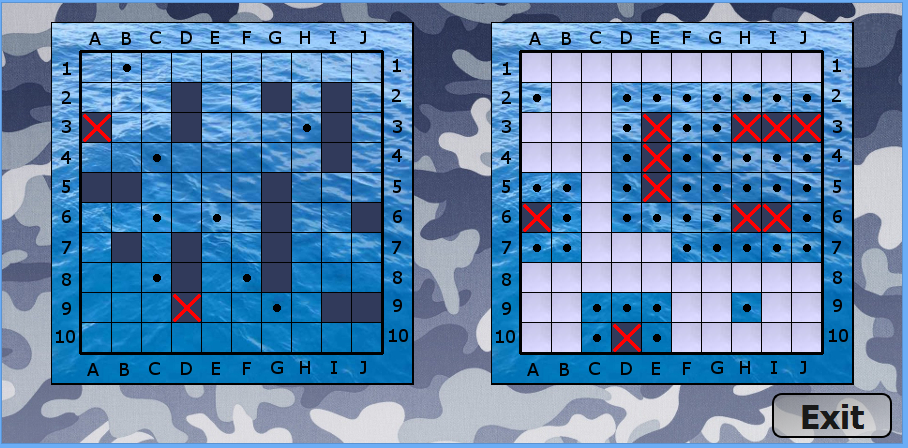
\includegraphics[scale=0.5]{screen/GUI_game_process.png}
		\caption{Игровой процесс} 
		\label{pic:pic_name} % название для ссылок внутри кода
	\end{center}
\end{figure}

На рис.11 показан пример того, как могут выглядеть поля во время игры.

\begin{figure}[H]
	\begin{center}
		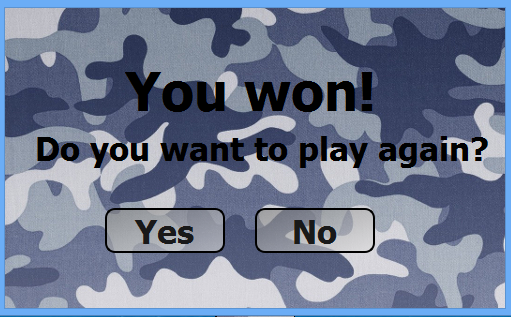
\includegraphics[scale=0.5]{screen/GUI_winner.png}
		\caption{Вывод победителя} 
		\label{pic:pic_name} % название для ссылок внутри кода
	\end{center}
\end{figure}

После того, как все корабли одного из полей будут потоплены, в отдельном окне отобразится победитель игры.

\subsection{Выводы}

В данном разделе были описаны все классы, выделенные в процессе работы над проектом. Также были сделаны снимки экрана, демонстрирующие работу консольного и графического приложений.

\section{Процесс обеспечения качества и тестирование}

\subsection{Просмотр кода и демонстрации}

Для обнаружения ошибок в коде программы один раз был проведен просмотр кода, замечания по которому практически полностью исправлены. Кроме того, были осуществлены 2 демонстрации, во время проведения которых были найдены ошибки в работе программы. Все замечания по демонстрациям также исправлены.

\subsection{Тестирование}

Для проверки работы библиотеки использовались автоматические тесты, покрывающие основную функциональность ядра. Также в процессе разработки приложения проводилось ручное тестирование программы.

\subsection{Выводы}

В данном разделе описаны просмотр кода и демонстрации, проведенные во время разработки приложения. Также рассказано о процессе тестирования работы программы. 

\section{Выводы}

Во время разработки приложения был значительно увеличен объем знаний, касаемых работы с языком программирования С++. Были изучены раннее неизвестные возможности С++ и лучше усвоены принципы объектно-ориентированного программирования. Кроме того, стали известны особенности стандарта С++11, а также основные паттерны проектирования. Помимо этого, был получен опыт в создании графического приложения с использованием библиотеки Qt.  
 

Результатом работы над проектом стала рабочая программа, позволяющая пользователям играть в Морской бой, используя при этом консоль или графичекое приложение. 

\section{Приложение 1}

\captionof{lstlisting}{game.h}
\lstinputlisting{../sources/Core/game.h}
\parindent=1cm

\captionof{lstlisting}{game.cpp}
\lstinputlisting{../sources/Core/game.cpp}
\parindent=1cm

\captionof{lstlisting}{field.h}
\lstinputlisting{../sources/Core/field.h}
\parindent=1cm

\captionof{lstlisting}{field.cpp}
\lstinputlisting{../sources/Core/field.cpp}
\parindent=1cm

\captionof{lstlisting}{ship.h}
\lstinputlisting{../sources/Core/ship.h}
\parindent=1cm

\captionof{lstlisting}{ship.cpp}
\lstinputlisting{../sources/Core/ship.cpp}
\parindent=1cm

\captionof{lstlisting}{cell.h}
\lstinputlisting{../sources/Core/cell.h}
\parindent=1cm

\captionof{lstlisting}{cell.cpp}
\lstinputlisting{../sources/Core/cell.cpp}
\parindent=1cm

\captionof{lstlisting}{main.cpp}
\lstinputlisting{../sources/Console/main.cpp}
\parindent=1cm

\captionof{lstlisting}{menu.cpp}
\lstinputlisting{../sources/Console/menu.cpp}
\parindent=1cm

\captionof{lstlisting}{application.h}
\lstinputlisting{../sources/Console/application.h}
\parindent=1cm

\captionof{lstlisting}{application.cpp}
\lstinputlisting{../sources/Console/application.cpp}
\parindent=1cm

\captionof{lstlisting}{main.cpp}
\lstinputlisting{../sources/GUI/main.cpp}
\parindent=1cm

\captionof{lstlisting}{mainwindow.h}
\lstinputlisting{../sources/GUI/mainwindow.h}
\parindent=1cm

\captionof{lstlisting}{mainwindow.cpp}
\lstinputlisting{../sources/GUI/mainwindow.cpp}
\parindent=1cm

\captionof{lstlisting}{gamewindow.h}
\lstinputlisting{../sources/GUI/gamewindow.h}
\parindent=1cm

\captionof{lstlisting}{gamewindow.cpp}
\lstinputlisting{../sources/GUI/gamewindow.cpp}
\parindent=1cm

\captionof{lstlisting}{resultwindow.h}
\lstinputlisting{../sources/GUI/resultwindow.h}
\parindent=1cm

\captionof{lstlisting}{resultwindow.cpp}
\lstinputlisting{../sources/GUI/resultwindow.cpp}
\parindent=1cm

\section{Приложение 2}


\end{document}